\documentclass[10pt,conference]{IEEEtran}

\usepackage{amsmath,amssymb}
\usepackage{booktabs}
\usepackage[T1]{fontenc}
\usepackage[utf8]{inputenc}
\usepackage{graphicx}
\usepackage{pgfplots}
\usepackage{tabularx}
\usepackage{tikz}
\usepackage{url}
\usepackage{hyperref}
\usetikzlibrary{arrows.meta,positioning,shapes.geometric,fit}
\pgfplotsset{compat=1.18}

\title{Request-Rooted Orchestration for Mixed Human-AI Fulfillment}

\author{
\IEEEauthorblockN{Draft Manuscript}
\IEEEauthorblockA{Boreal Network}
}

\begin{document}

\maketitle

\begin{abstract}
AI-capable systems are increasingly used to perform external digital work, but current software stacks fragment demand capture, matching, execution, proof, and payment across chat interfaces, marketplaces, task trackers, and provider-specific tools. This fragmentation is especially costly when work begins as an ambiguous request and is fulfilled by mixed human and AI participants across both digital and embodied steps. Existing agent planners are often biased toward callable digital tools and therefore under-specify or omit work that requires physical presence, local access, field inspection, witnessed handoff, or other human-executed verification. We describe this failure mode as generative plan collapse: the tendency to produce plans that are coherent in language but incomplete in real-world executability.

We present a request-rooted orchestration model for mixed human-AI fulfillment in which a single durable \texttt{Request} persists across intake, routing, \texttt{Commitment}, \texttt{Fulfillment}, \texttt{Artifact} delivery, \texttt{Transaction} state, and append-only \texttt{RequestEvent} history. The model separates current summary state from durable ledger history and distinguishes ephemeral execution signals such as typing, token streams, progress ticks, and runtime logs from business-meaningful state transitions. It also preserves explicit representation of embodied constraints, human-presence requirements, and verification obligations instead of allowing planners to optimize them away.

We implement the model in Boreal Network as a docs-first, machine-readable contract stack with JSON Schema, OpenAPI, event contracts, deterministic fixtures, and an evaluation harness for extraction, matching, planning, and mutation safety. We further define a lead-first orchestration policy that matches a primary \texttt{Supply} before decomposing work into \texttt{FulfillmentStep} sub-work, aiming to reduce over-decomposition, false completion, and premature execution. In a deterministic four-scenario benchmark spanning one digital and three embodied cases, the request-rooted baseline achieves 100\% contract pass, 100\% embodied-step recall, and 0\% false completion, while task-first and direct-tool baselines expose distinct failure modes: complete over-decomposition in the former and 100\% embodied-collapse plus 75\% false completion in the latter. A complementary live-model study across five OpenAI-routed models and two frozen prompt presets shows that current models can recover the correct lead and stay inside safe action bands while still failing exact canonical conformance and under-specifying verification fields. This paper contributes a durable object model for request-native work systems, a framing of generative plan collapse in embodied and digital fulfillment, and an artifact-backed methodology for evaluating continuity, traceability, human routing, and approval safety in external work orchestration.
\end{abstract}

\section{Introduction}
Current AI systems can interpret requests, generate digital outputs, browse the web, and call APIs. Those capabilities are often enough to produce plausible-looking work artifacts. They are not, by themselves, enough to model the full path from ambiguous demand to verified completion. Real work routinely spans clarification, pricing, approval, execution, proof, delivery, and payout. It may also require local access, onsite presence, witnessed handoff, hardware interaction, or field inspection. When those steps are not represented explicitly, the system can still produce polished outputs while failing to capture the actual work needed for completion.

This gap matters more as AI systems move from advisory roles into fulfillment roles. A buyer does not only need a generated answer. The buyer needs a completed outcome, often produced by a mix of humans, agents, tools, and runtimes. Existing stacks tend to fragment this lifecycle across separate surfaces: chat handles intake, a planner generates tasks, a marketplace or directory handles matching, a tracker holds status, and payment systems sit elsewhere. The result is weak continuity. Context drifts across surfaces, approval boundaries blur, and proof of completion is often reduced to narrative summaries rather than durable evidence. Market signals from major work platforms and AI vendors reinforce the importance of this gap: external AI-related work is already monetizing, marketplaces are moving toward fulfillment infrastructure, and enterprise buyers increasingly want systems that connect execution across tools rather than isolated point solutions \cite{upwork_q4_2025,openai_enterprise_ai_2026,microsoft_frontier_suite_2026}.

The problem becomes sharper when fulfillment includes embodied work. Many planners are biased toward the actions they can call directly. If a system can browse a website, produce a checklist, and write a report, it may silently substitute those steps for the real requirement of visiting a site, inspecting an environment, or witnessing a handoff. In other words, the planner overfits to digital executability. This can create outputs that are coherent in language while remaining incomplete in real-world terms.

We argue that a better systems primitive for this setting is a durable request-rooted model. In our approach, one \texttt{Request} persists across intake, routing, \texttt{Commitment}, \texttt{Fulfillment}, proof, and payout. This design treats the request as the canonical work thread rather than as a temporary precursor to separate planner, marketplace, or execution objects. It also allows the system to keep digital and embodied steps inside one accountable lifecycle rather than forcing the physical parts of the work outside the model.

This paper uses Boreal Network as the concrete artifact for exploring that claim. Boreal defines a docs-first and machine-readable contract stack centered on one durable \texttt{Request}, explicit \texttt{Supply}, commercial and approval boundaries through \texttt{Commitment}, execution truth through \texttt{Fulfillment}, proof through \texttt{Artifact}, payment state through \texttt{Transaction}, and append-only history through \texttt{RequestEvent}. Within that model we also define a lead-first orchestration rule: match the lead first, plan the work second, and decompose only when needed.

The paper makes three main contributions. First, it presents a request-rooted object model for mixed human-AI fulfillment that keeps demand, execution, and proof on one durable thread. Second, it identifies a practical failure mode in current agent planning, which we call generative plan collapse: the omission or weakening of required embodied work because the planner is biased toward digitally callable actions. Third, it outlines an artifact-backed evaluation methodology for comparing request-rooted orchestration against chat-first, task-first, and direct-tool baselines on continuity, verification, and false-completion risk.


\section{Problem}
Systems for AI-assisted work commonly inherit one of three weak defaults. The first is the chat-first default. In chat-first systems, a conversation thread captures user intent and model responses, but the commercial and execution structure of the work remains implicit. Pricing, approval, proof, and delivery often appear as plain messages rather than as durable state transitions. The second is the listing-first or marketplace-first default. In these systems, supply is modeled clearly, but demand is assumed to be already scoped. That assumption breaks when the buyer begins with an ambiguous request rather than a precise task description. The third is the task-first or tool-first default. These systems turn the request into a tree of steps early, usually shaped by the tools the system can access.

The task-first default creates a particularly important distortion. If the planner can call browser tools, APIs, search, and generation routines, it will often decompose the work according to those capabilities. Steps requiring local access, physical presence, field measurement, or witnessed completion are harder to represent and often harder to route. As a result, the planner may weaken or remove them. What remains is a plan optimized for what the system can execute digitally rather than for what the request actually requires.

\begin{table}[t]
\caption{Coordination defaults and dominant failure modes.}
\label{tab:coordination-defaults}
\centering
\footnotesize
\begin{tabularx}{\columnwidth}{p{1.45cm}p{1.75cm}X}
\toprule
Default & Root unit & Dominant failure mode \\
\midrule
Chat-first & Conversation thread & Weak approval, payment, and proof structure \\
Listing-first & Supply listing or posted task & Assumes demand is already scoped \\
Tool-first & Callable step & Omits non-digital or access-constrained work \\
Request-rooted & Durable request thread & Higher modeling cost, but preserves continuity and proof obligations \\
\bottomrule
\end{tabularx}
\end{table}

We describe this failure mode as \emph{generative plan collapse}. A plan has collapsed in this sense when it appears complete and actionable in language, but omits one or more execution-critical steps because those steps are embodied, access-constrained, or difficult to verify through the planner's native action surface. The collapse is not merely about low-quality generation. It is structural. The system is rewarded for producing a coherent plan inside its sandbox, even when the true completion path lies partly outside that sandbox.

Several examples illustrate the problem. An onsite property inspection may be replaced by a generated checklist and a summary template. A hardware or facility audit may be reframed as documentation review. A document pickup or witnessed dropoff may be reduced to an email draft. Field photography may be replaced by synthetic imagery or unverifiable stock references. A compliance visit may be summarized from remote assumptions rather than site-specific evidence. In each case, the planner still produces something that looks productive, but the work thread has drifted away from executability.

\begin{figure}[t]
\centering
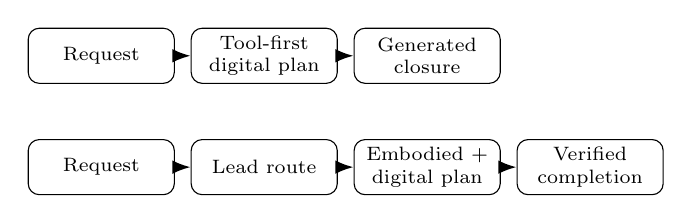
\begin{tikzpicture}[
  >=Latex,
  node distance=2mm,
  box/.style={draw, rounded corners, align=center, font=\scriptsize, minimum height=7mm, text width=1.75cm, inner sep=1.5pt},
  arrow/.style={->, thick}
]
\node[box] (r1) {Request};
\node[box, right=of r1] (p1) {Tool-first\\digital plan};
\node[box, right=of p1] (c1) {Generated\\closure};
\draw[arrow] (r1) -- (p1);
\draw[arrow] (p1) -- (c1);

\node[box, below=7mm of r1] (r2) {Request};
\node[box, right=of r2] (l2) {Lead route};
\node[box, right=of l2] (p2) {Embodied +\\digital plan};
\node[box, right=of p2] (v2) {Verified\\completion};
\draw[arrow] (r2) -- (l2);
\draw[arrow] (l2) -- (p2);
\draw[arrow] (p2) -- (v2);
\end{tikzpicture}
\caption{Generative plan collapse contrasted with request-rooted correction. The top lane optimizes for callable digital actions; the bottom lane preserves route and verification requirements before completion.}
\label{fig:collapse}
\end{figure}

This is not only a user-experience issue. It is also a systems integrity issue. When omitted embodied steps are not represented explicitly, the system loses the ability to enforce approvals, require the right kind of proof, or distinguish valid completion from narrative closure. The problem is therefore not simply that current planners are imperfect. It is that the surrounding object model often gives them no durable place to record what kind of work must happen, who must do it, where it must occur, or what evidence would count as completion.


\section{Formal Problem Setting}
We formalize the orchestration setting around one incoming request $q$. Let $q$ contain a brief, structured constraints, visibility policy, and proof obligations. Let $\mathcal{S}$ denote the set of candidate supplies available to respond. Each supply $s \in \mathcal{S}$ is characterized by capability features, trust features, geography or access constraints, and execution affordances. Those affordances may be purely digital, hybrid, or embodied.

The planner outputs a tuple $\pi(q) = (s^\star, P_q, V_q)$ where $s^\star$ is the selected lead supply, $P_q$ is the derived plan, and $V_q$ is the set of verification obligations that must be satisfied before completion. The key design choice is that $P_q$ is produced only after the lead route is fixed. This is the formal version of the lead-first rule.

We write the lead-selection rule as
\begin{equation}
\begin{aligned}
s^\star = \arg\max_{s \in \mathcal{S}} \Big(
&\lambda_{\text{cap}}\phi_{\text{cap}}(q,s)+
\lambda_{\text{geo}}\phi_{\text{geo}}(q,s) \\
&+\lambda_{\text{emb}}\phi_{\text{emb}}(q,s)+
\lambda_{\text{trust}}\phi_{\text{trust}}(q,s) \\
&-\lambda_{\text{gap}}\phi_{\text{gap}}(q,s)
\Big),
\end{aligned}
\end{equation}
where the $\phi$ terms measure capability fit, geographic fit, embodied-execution fit, trust compatibility, and missing-constraint gap respectively. The embodied term is important: a plan should not score highly simply because a supply can generate plausible digital outputs. It should score highly only if the supply can execute the required work mode. This is aligned in spirit with grounding plans in executable affordances rather than in language-only plausibility \cite{ahn2022saycan}.

Let $E_q$ denote the set of embodied steps actually required by request $q$, and let $\hat{E}_q$ denote the subset of embodied steps represented in the generated plan. We define embodied-step recall as
\begin{equation}
\operatorname{ER}(q)=\frac{|E_q \cap \hat{E}_q|}{|E_q|}.
\end{equation}
We then define generative plan collapse for a request as the complement
\begin{equation}
\operatorname{GPC}(q)=1-\operatorname{ER}(q).
\end{equation}
This captures one of the paper's core failure modes: the more required embodied work is omitted from the plan, the greater the collapse.

Finally, let $A_q$ denote the realized artifact set attached to the request and fulfillment lane. We define a false-completion indicator as
\begin{equation}
\operatorname{FC}(q)=
\mathbb{I}\left[
\texttt{completed}(q)\ \land\
\big(E_q \nsubseteq \hat{E}_q\ \lor\ V_q \nsubseteq A_q\big)
\right].
\end{equation}
In words, a request has false completion if the system reaches a completed state while either required embodied steps were not preserved in the plan or required verification obligations were not realized in artifacts. These definitions give the paper an evaluable target that goes beyond fluency or plan length.


\section{Design Requirements}
To address this problem, a work-orchestration system must satisfy requirements that are not well covered by chat-only or tool-first abstractions. First, it must preserve one durable work thread from demand intake to completion. A buyer should not lose continuity when the workflow moves from clarification to routing, from routing to approval, or from approval to execution. Second, it must represent commercial boundaries explicitly. Approval, pricing, and payment are not side messages. They are part of the work lifecycle and must be modeled as first-class state.

Third, the system must support mixed participation. Real requests may involve human specialists, agents, tools, organizations, and local runtimes in one fulfillment path. The model therefore needs a durable way to represent both who owns the request and which supply-side capabilities respond to it. Fourth, the system must preserve auditable history. Current summary state is useful for product surfaces, but the durable record of what happened, who changed it, and which proof artifacts were attached should remain reconstructible.

Fifth, the system must support proof-bearing completion rather than generated closure. Completion should depend on evidence appropriate to the work mode. For digital work, this may involve code, documents, URLs, or execution traces. For embodied work, it may involve photographs, signatures, geostamped check-ins, access logs, receipts, or witness-confirmed handoffs. The model must therefore represent proof obligations without forcing all proof data inline onto the root object.

Sixth, the system must represent embodied constraints explicitly. These include location requirements, travel or geography constraints, time windows, access dependencies, safety constraints, trust requirements, and the need for human presence. If those requirements exist only in freeform text or remain implicit in the buyer's message, the planner will be tempted to optimize them away. The representation does not have to introduce a new root object, but it does need durable fields or derived structures that allow the system to reason about embodied execution honestly.

Finally, the system must resist premature decomposition. If decomposition happens before a credible lead route is known, the planner is likely to produce generic task trees or tool-shaped work breakdowns. A realistic orchestration system should establish the primary execution path first, then derive bounded sub-work around that path. This motivates the lead-first rule that we use later in the paper.


\section{Request-Rooted Model}
Our model uses \texttt{Request} as the durable demand-side root. A request begins from need: someone needs work done and opens a thread that may still be ambiguous. That thread can then survive clarification, routing, approval, funding, execution, proof, delivery, and payout without leaving the same durable object family. This is a deliberate contrast to models that begin with a catalog item, a chat session, or a detached task tree.

\begin{figure}[t]
\centering
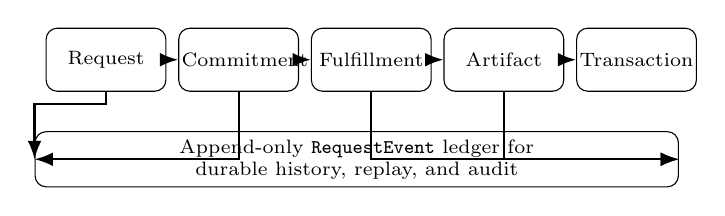
\begin{tikzpicture}[
  >=Latex,
  node distance=1.5mm,
  box/.style={draw, rounded corners, align=center, font=\scriptsize, minimum height=8mm, text width=1.45cm, inner sep=1pt},
  ledger/.style={draw, rounded corners, align=center, font=\scriptsize, minimum height=7mm, text width=8.1cm, inner sep=1pt},
  arrow/.style={->, thick}
]
\node[box] (req) {Request};
\node[box, right=of req] (com) {Commitment};
\node[box, right=of com] (ful) {Fulfillment};
\node[box, right=of ful] (art) {Artifact};
\node[box, right=of art] (txn) {Transaction};
\draw[arrow] (req) -- (com);
\draw[arrow] (com) -- (ful);
\draw[arrow] (ful) -- (art);
\draw[arrow] (art) -- (txn);
\node[ledger, below=5mm of com, xshift=1.5cm] (evt) {Append-only \texttt{RequestEvent} ledger for durable history, replay, and audit};
\draw[arrow] (req.south) -- ++(0,-1.6mm) -| (evt.west);
\draw[arrow] (com.south) -- ++(0,-1.6mm) |- (evt.west);
\draw[arrow] (ful.south) -- ++(0,-1.6mm) |- (evt.east);
\draw[arrow] (art.south) -- ++(0,-1.6mm) |- (evt.east);
\end{tikzpicture}
\caption{Request-rooted lifecycle with adjacent durable objects. The request remains the demand-side root while commitment, fulfillment, proof, payment, and durable history stay attached to the same work thread.}
\label{fig:lifecycle}
\end{figure}

The surrounding objects preserve explicit boundaries. \texttt{Actor} represents participant identity. \texttt{Supply} represents published capability that can be matched, invited, hired, or routed. \texttt{RequestParticipant} makes actor-to-request relationships explicit rather than hiding them in ad hoc arrays. \texttt{Commitment} represents a commercial or approval boundary such as a proposal, assignment, or accepted route. \texttt{Fulfillment} represents an execution lane that has actually started. \texttt{FulfillmentStep} represents bounded sub-work under that lane. \texttt{Artifact} represents output or proof. \texttt{Transaction} represents payment or settlement state. \texttt{RequestEvent} provides append-only history.

This object split matters because it allows continuity without overloading the request root. The request stores current summary state, such as the brief, visibility, high-level constraints, current status, and active references. It does not need to store every event, artifact, or payment update inline. Full history lives in the event ledger and adjacent durable objects. This separation keeps the root object readable while still allowing replay, audit, and projection rebuilds.

The request-rooted model is especially useful for mixed digital and embodied work because it provides one durable place to keep the execution thread honest. A request for a local compliance visit, for example, does not become a different class of business object just because some steps happen onsite. The same request can hold the brief, the chosen supply, the accepted commercial boundary, the active fulfillment, the inspection artifacts, and the settlement records. This makes it harder for the planner or interface to treat embodied work as outside the system's concern.

The model also preserves a clean default for sub-work. Worker-generated decomposition should become \texttt{FulfillmentStep} rather than a new root request, unless there is a true boundary of separate ownership, separate funding, separate market routing, or separate review. This rule is important because many AI systems implicitly create new tasks whenever they decompose work. In our model, decomposition is subordinate to the accepted fulfillment lane, not a justification for forking business truth.


\section{Core Invariants}
The request-rooted model depends on a small set of invariants. The first invariant is that one \texttt{Request} should survive the lifecycle by default. Intake, routing, approval, execution, proof, and payout should remain attached to the same demand-side thread unless there is a real boundary of separate funding, separate ownership, separate market routing, or separate review. This prevents the system from scattering business truth across disconnected artifacts simply because the work became more detailed.

The second invariant is that internal decomposition does not imply a new business root. Sub-work created by a worker, planner, or runtime should become \texttt{FulfillmentStep} under an existing \texttt{Fulfillment}. This keeps execution decomposition subordinate to the accepted lane rather than letting every subtask spawn a new request or pseudo-order object. The rule matters because AI systems often create extra task objects by default, which makes lifecycle reasoning and payment accountability harder.

The third invariant is that commitment and fulfillment remain distinct. Selecting a route, accepting a proposal, or approving commercial terms is not the same as starting execution. Public or cross-actor work should preserve a \texttt{Commitment} gate before \texttt{Fulfillment} begins. Private owner-controlled shortcuts may exist in bounded cases, but those shortcuts should remain explicit exceptions rather than becoming the silent default.

The fourth invariant is that current summary state and full history are separated. The request root should store current truth such as the brief, visibility, high-level constraints, and active references. The append-only ledger and adjacent durable objects should store the full history of what actually happened. This protects both readability and auditability.

The fifth invariant is that completion must be evidenced according to execution mode. Digital work may close through document, code, or object references. Embodied work may require photographs, signatures, access logs, witness confirmation, or other field-specific proof. The system should therefore validate completion against proof obligations rather than against narrative closure alone.


\section{Lead-First Orchestration}
The orchestration rule in Boreal is simple: match the lead first, plan the work second, and decompose only when needed. This rule is intentionally conservative. It rejects the assumption that the first useful response to an ambiguous request is always a task tree. In many requests, especially higher-complexity ones, the decisive question is not ``what are the steps'' but ``who or what should lead the work.''

Lead-first orchestration has two benefits. The first is quality. Once a credible lead \texttt{Supply} is identified, the system can shape the rest of the plan around a realistic execution path. The second is safety. Premature decomposition creates pressure to allocate sub-work before approval, before commercial boundaries are clear, and before the system knows whether the fulfillment path is digital, embodied, or hybrid.

This matters directly for embodied work. Suppose a request involves an onsite visit and a follow-up report. A tool-first planner may start by drafting a checklist, an email template, and a report outline because those are callable outputs. A lead-first planner should instead ask whether the request requires local presence, whether a field-capable supply exists in the right geography, and whether the owner has specified the access and verification conditions. Only after that lead route is credible should the system derive sub-work such as documentation, summary writing, or operator review.

The same logic applies to hybrid work. A local human may need to perform inspection, pickup, installation, or witness tasks, while an agent or tool handles background research, document assembly, or structured reconciliation. Lead-first orchestration allows the digital steps to support the embodied path rather than silently replacing it. In this sense, the rule is not only a planning heuristic. It is a guardrail against tool-shaped underplanning.


\section{Embodied Work Representation}
Embodied work includes any fulfillment step that depends on physical presence, place-specific context, local access, real-world timing, or human witnessing. Common examples include onsite visits, field inspection, pickup or dropoff, event attendance, device or environment interaction, in-person verification, and handoff that requires a signature or observed confirmation. These steps differ from pure digital tasks because they cannot be reduced to generation quality alone. Their correctness depends on where, when, and by whom the work occurred.

For that reason, an orchestration model should represent embodied work explicitly rather than treating it as a weak annotation on a generic task. At minimum, the system should be able to distinguish among execution modalities such as remote digital work, remote synchronous interaction, onsite visit, field inspection, pickup or dropoff, human review, and witnessed handoff. It should also be able to represent planning constraints such as geography, time window, access dependency, safety requirement, or required proof type.

These requirements do not necessarily imply a new root object. They can be represented through canonical request fields, structured matching criteria, fulfillment-step metadata, or proof requirements attached to the execution lane. The crucial point is that the information must be durable enough to affect routing and validation. If the need for onsite presence exists only in one freeform paragraph, it is easy for a planner to ignore it and still appear productive.

Explicit embodied representation also changes how supply is modeled. A supply should not be described only by abstract capability labels. It should be possible to express whether a supply can provide local presence, what geography it can serve, whether it can perform inspections or witness tasks, whether it can handle access-constrained sites, and what proof surfaces it can produce. This lets the system distinguish a strong digital analyst from a field-capable operator even if both could generate polished reports.

Finally, explicit representation changes completion rules. A summary that says ``inspection completed'' is not the same as an inspection artifact. A generated checklist is not the same as a geostamped site photo, a witness signature, or a time-bound access log. The model should therefore require proof appropriate to the execution mode. Otherwise, the system cannot distinguish real completion from narrative closure.


\section{Durable and Ephemeral Boundaries}
One of the risks in mixed human-AI orchestration is confusing visible activity with durable progress. Many runtime signals are useful for operator awareness: typing indicators, token streams, progress ticks, heartbeats, presence updates, and transient logs can all help users understand that execution is happening. However, those signals are not durable business truth by default. Storing them as if they were equivalent to business events creates noisy history and makes it harder to identify what actually mattered.

In Boreal, this distinction is represented by separating ephemeral transport signals from durable request history. Ephemeral signals may travel through local IPC, browser bridges, streaming transport, or peer channels. Durable history is promoted only when the outcome has business meaning. Examples include a fulfillment state change, a blocker summary, a delivery-ready summary, an artifact reference, or a payment-relevant fact. This keeps the append-only ledger meaningful rather than turning it into a dump of every token and heartbeat.

The distinction is even more important for embodied work. A stream of progress messages does not prove that a site was visited. A verbose model trace does not prove that a human witness observed a handoff. If the system treats runtime chatter as equivalent to completion evidence, it will make generative plan collapse harder to detect. Durable proof has to be attached through the right object family, typically \texttt{Artifact} plus corresponding \texttt{RequestEvent} or \texttt{Fulfillment} transitions.

This separation also improves system design discipline. Interfaces can remain responsive and transparent without inflating the durable history model. Operators can still see transient execution signals, but business state remains tied to explicit promotions. In other words, the model supports visibility without sacrificing auditability.


\section{Boreal Network Artifact}
Boreal Network serves as the concrete artifact for this paper. It is not presented as a finished production system that already proves every downstream claim. Rather, it provides a structured and inspectable baseline for studying request-rooted orchestration. The artifact is docs-first: canonical object meanings, lifecycle rules, event semantics, request-processing rules, and governance constraints are defined in root documentation before or alongside implementation work \cite{boreal_repo_2026,boreal_network_thesis_2026,boreal_request_processing_2026}.

The artifact also includes machine-readable layers. Canonical object shapes are represented through JSON Schema. HTTP surfaces are represented through OpenAPI. Durable request activity and related event channels are represented through event contracts. Deterministic fixtures provide canonical request threads and planner or matcher scenarios. An eval runner checks extraction, routing, matching, planning, and mutation-safety expectations against those fixtures. Together, these layers make the system more than a prose concept. They provide a reproducible contract baseline that can be inspected, extended, and tested.

This structure is helpful for research because it separates semantic claims from implementation-local behavior. The object model and invariants can be discussed directly. The planner rules can be evaluated against fixed scenarios. The lifecycle and mutation boundaries can be tested without requiring that every future product surface or peer runtime already be fully built. In that sense, Boreal is a suitable artifact for studying how a request-rooted model behaves even before large-scale deployment data exists.

For the current paper, the artifact should be read as a prototype baseline plus evaluation substrate. The research claims are therefore bounded: Boreal demonstrates a coherent durable model, a contract stack, and an evaluation direction. It does not, by itself, establish market-wide superiority, complete empirical validation, or coverage of every class of embodied work. Those stronger claims belong to future studies.


\section{Case Studies}
To make the model concrete, the paper should analyze both digital-heavy and embodied or hybrid scenarios. A useful digital-heavy baseline already exists in Boreal's deterministic fixture set: a support-triage automation request in which one buyer opens a request, one supply responds, one commitment is accepted, fulfillment proceeds, artifacts are delivered, and settlement closes on the same durable thread. This scenario is valuable because it shows that the model handles an AI-heavy or operations-heavy request without needing to invent secondary root objects.

However, the embodied gap appears more clearly in hybrid scenarios. Consider an onsite property inspection that also requires a structured written report. A tool-first system can readily generate the report template and checklist, but it may omit the actual visit, the access coordination, the time window, and the evidence obligations. In a request-rooted model, those conditions remain attached to the request and shape both supply selection and completion validation. The digital report is a supporting artifact, not a substitute for the inspection itself.

Another useful scenario is a local inventory audit with photo evidence and reconciliation. Here the fulfillment path mixes physical presence with digital follow-up. A field-capable human may count or inspect items onsite, while an agent or tool normalizes records, produces summaries, or highlights discrepancies. The key point is that the digital support lane should remain attached to, and subordinate to, the embodied execution lane rather than silently replacing it.

Case studies of this kind help distinguish between two superficially similar systems: one that generates convincing documents about work and one that keeps the work thread honest enough to route, verify, and settle the actual underlying task. That distinction is central to the paper's claim.


\section{Evaluation and Preliminary Results}
The evaluation goal is not only to test whether the system can produce fluent plans. It is to test whether the system preserves executability, approval safety, and proof obligations across both digital and embodied work. We operationalize this goal as a deterministic artifact benchmark built from canonical fixtures plus authored baseline outputs in the repository \cite{boreal_request_processing_benchmark_2026,boreal_request_eval_fixtures_2026}. The current benchmark contains four scenarios: one digital high-complexity migration request and three embodied requests covering onsite inspection, hardware installation verification, and pickup with witnessed handoff.

Each scenario is evaluated against three system families. \emph{Request-rooted} models the intended Boreal policy: lead-first matching, explicit embodied execution modes, and approval-safe next actions. \emph{Task-first} models a planner that decomposes immediately into many subtasks before securing the right lead and before preserving bounded phase structure. \emph{Direct-tool} models a digitally callable baseline that prefers remote generation and tool invocation, even when the request requires onsite execution or field verification. These are controlled benchmark output packs, not claims about live production traces.

We report nine aggregate metrics from the benchmark runner. \emph{Contract pass rate} measures whether a system satisfies the full fixture contract. \emph{Lead top-1 accuracy} and \emph{Recall@3} measure routing quality. \emph{Over-decomposition rate} measures whether the system exceeds the expected phase bounds or abandons the no-microtask invariant. \emph{Forbidden mutation rate} measures unsafe movement into fulfillment before the fixture allows it. \emph{Embodied-step recall} measures whether required physical execution modes remain present in the plan. \emph{Generative plan collapse} is the complement of embodied-step recall on embodied scenarios. \emph{Verification completeness} measures whether required proof claims remain represented. \emph{False-completion rate} measures whether the workflow moves toward fulfillment or closure while required embodied or verification obligations remain unresolved.

The benchmark cleanly separates the three planning styles. The request-rooted baseline achieves 100\% contract pass, 100\% lead top-1 accuracy, 100\% embodied-step recall, 100\% verification completeness, and 0\% false completion. The task-first baseline still recovers the correct lead within the top three candidates on every scenario, but it drops to 50\% top-1 accuracy, reaches 100\% over-decomposition, and preserves only 66.7\% embodied-step recall. The direct-tool baseline avoids over-decomposition only because it largely stops planning; on this benchmark it records 0\% lead top-1 accuracy, 100\% forbidden mutation, 0\% embodied-step recall, 27.8\% verification completeness, and 75\% false completion. This result is important because it shows that low decomposition count alone is not evidence of good orchestration. A system can avoid task explosion by collapsing the work into unsafe or unverifiable digital-only outputs.

% Generated by tests/contracts/run-request-processing-benchmark.mjs
\begin{table*}[t]
\centering
\caption{Deterministic request-processing benchmark across 4 scenarios. Higher is better for pass rate, lead accuracy, embodied recall, and verification completeness. Lower is better for over-decomposition, forbidden mutation, generative plan collapse, and false completion.}
\label{tab:deterministic-benchmark}
\resizebox{\textwidth}{!}{%
\begin{tabular}{lccccccccc}
\toprule
System & Pass Rate & Lead Top-1 & Recall@3 & Over-Decomp & Forbidden Mutation & Embodied Recall & Collapse & Verification & False Completion \\
\midrule
Direct-Tool & 0.0\% & 0.0\% & 0.0\% & 0.0\% & 100.0\% & 0.0\% & 100.0\% & 27.8\% & 75.0\% \\
Request-Rooted & 100.0\% & 100.0\% & 100.0\% & 0.0\% & 0.0\% & 100.0\% & 0.0\% & 100.0\% & 0.0\% \\
Task-First & 0.0\% & 50.0\% & 100.0\% & 100.0\% & 0.0\% & 66.7\% & 33.3\% & 72.2\% & 0.0\% \\
\bottomrule
\end{tabular}
}
\end{table*}

\begin{figure}[t]
\centering
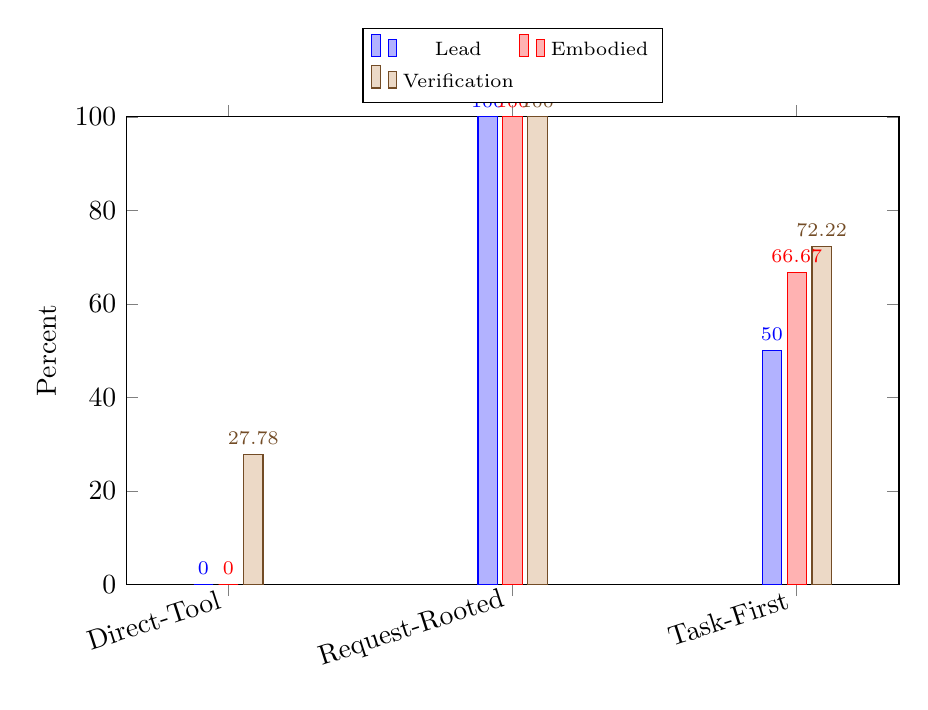
\begin{tikzpicture}
\begin{axis}[
  ybar,
  bar width=7pt,
  width=0.94\columnwidth,
  height=0.62\columnwidth,
  ymin=0,
  ymax=100,
  ylabel={Percent},
  symbolic x coords={Direct-Tool,Request-Rooted,Task-First},
  xtick=data,
  x tick label style={rotate=18, anchor=east},
  legend style={font=\scriptsize, at={(0.5,1.03)}, anchor=south, legend columns=2},
  nodes near coords,
  every node near coord/.append style={font=\scriptsize},
  enlarge x limits=0.18
]
\addplot coordinates {(Direct-Tool, 0) (Request-Rooted, 100) (Task-First, 50)};
\addplot coordinates {(Direct-Tool, 0) (Request-Rooted, 100) (Task-First, 66.66666666666666)};
\addplot coordinates {(Direct-Tool, 27.777777777777775) (Request-Rooted, 100) (Task-First, 72.22222222222221)};
\legend{Lead, Embodied, Verification}
\end{axis}
\end{tikzpicture}
\caption{Outcome quality on the deterministic benchmark. The request-rooted baseline preserves both routing quality and embodied verification fidelity, while the direct-tool baseline collapses on physical-work retention.}
\label{fig:deterministic-benchmark}
\end{figure}


To move beyond authored baselines, we also ran a live-model benchmark through the Boreal web workspace's AI Gateway path using frozen prompt presets, stable local scoring, and recorded request-response metadata \cite{boreal_request_live_benchmark_runner_2026,boreal_request_live_benchmark_results_2026}. The study evaluated five OpenAI-routed models under two prompt families: \emph{neutral\_contract\_v2}, which exposes the output contract without Boreal-specific framing, and \emph{boreal\_canon\_v2}, which adds the request-rooted lead-first rules while keeping the same canonical output vocabulary. The live runner records call success, parse success, exact contract pass, lead accuracy, safe action acceptability, required-role coverage, semantic embodied retention, and semantic verification retention. This split matters because provider access failure, JSON formatting failure, and planning failure are different phenomena and should not be collapsed into one score.

% Generated by apps/web/scripts/run-request-processing-live-benchmark.ts
\begin{table*}[t]
\centering
\small
\setlength{\tabcolsep}{4pt}
\caption{Live request-processing benchmark over frozen prompt presets and real model calls. Exact contract pass remained brittle, so this export emphasizes availability, parse reliability, safe action choice, role preservation, semantic embodied retention, and semantic verification retention.}
\label{tab:live-request-processing-benchmark}
\resizebox{\textwidth}{!}{%
\begin{tabular}{lcccccccccc}
\toprule
System & Call & Parse & Exact Pass & Lead Top-1 & Policy Accept & Required Roles & Exact Embodied & Semantic Embodied & Semantic Verification & False Completion \\
\midrule
gpt-4.1-nano + Neutral & 100.0\% & 75.0\% & 0.0\% & 100.0\% & 100.0\% & 100.0\% & 0.0\% & 83.3\% & 33.3\% & 0.0\% \\
gpt-4.1-nano + Boreal & 100.0\% & 75.0\% & 0.0\% & 100.0\% & 66.7\% & 83.3\% & 0.0\% & 75.0\% & 25.0\% & 0.0\% \\
gpt-5.4-nano + Neutral & 100.0\% & 100.0\% & 0.0\% & 100.0\% & 100.0\% & 87.5\% & 16.7\% & 83.3\% & 33.3\% & 0.0\% \\
gpt-5.4-nano + Boreal & 100.0\% & 100.0\% & 0.0\% & 100.0\% & 100.0\% & 87.5\% & 0.0\% & 100.0\% & 33.3\% & 0.0\% \\
gpt-5-mini + Neutral & 100.0\% & 0.0\% & 0.0\% & n/a & n/a & n/a & n/a & n/a & n/a & n/a \\
gpt-5-mini + Boreal & 100.0\% & 0.0\% & 0.0\% & n/a & n/a & n/a & n/a & n/a & n/a & n/a \\
o4-mini + Neutral & 100.0\% & 50.0\% & 0.0\% & 100.0\% & 100.0\% & 100.0\% & 0.0\% & 100.0\% & 50.0\% & 0.0\% \\
o4-mini + Boreal & 100.0\% & 50.0\% & 0.0\% & 100.0\% & 100.0\% & 100.0\% & 0.0\% & 50.0\% & 0.0\% & 0.0\% \\
gpt-5-pro + Neutral & 0.0\% & 0.0\% & 0.0\% & n/a & n/a & n/a & n/a & n/a & n/a & n/a \\
gpt-5-pro + Boreal & 0.0\% & 0.0\% & 0.0\% & n/a & n/a & n/a & n/a & n/a & n/a & n/a \\
\bottomrule
\end{tabular}
}
\end{table*}


\begin{figure}[t]
\centering
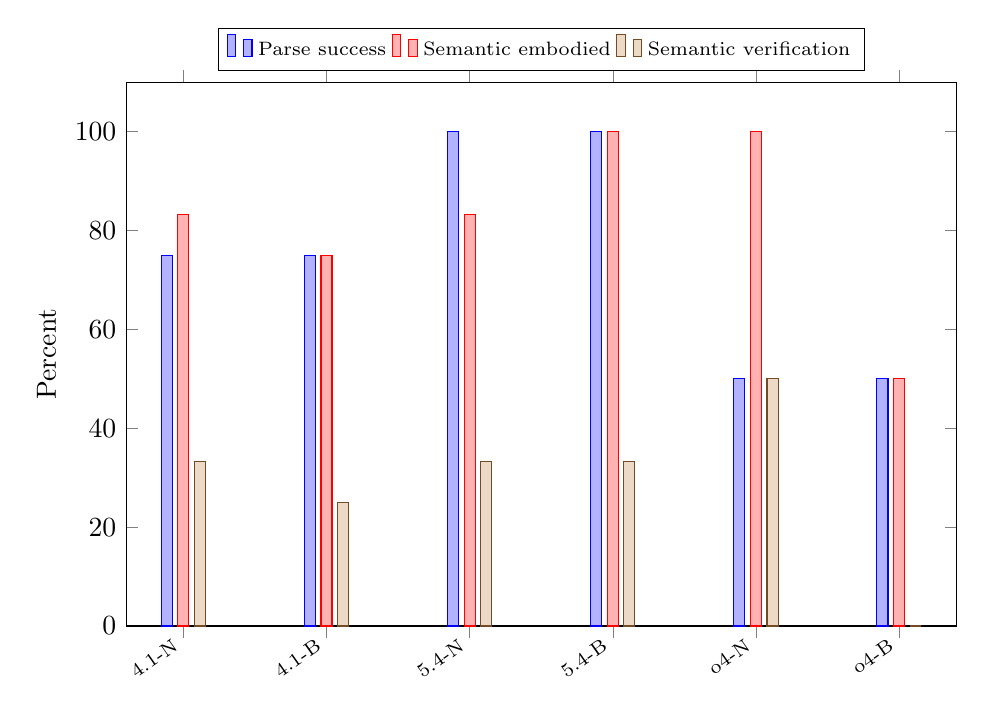
\begin{tikzpicture}
\begin{axis}[
  width=\columnwidth,
  height=0.7\columnwidth,
  ybar,
  bar width=4pt,
  ymin=0,
  ymax=110,
  ylabel={Percent},
  symbolic x coords={4.1-N,4.1-B,5.4-N,5.4-B,o4-N,o4-B},
  xtick=data,
  xticklabel style={rotate=35,anchor=east,font=\scriptsize},
  legend style={font=\scriptsize,at={(0.5,1.02)},anchor=south,legend columns=3},
  enlarge x limits=0.08
]
\addplot coordinates {(4.1-N,75) (4.1-B,75) (5.4-N,100) (5.4-B,100) (o4-N,50) (o4-B,50)};
\addplot coordinates {(4.1-N,83.3) (4.1-B,75) (5.4-N,83.3) (5.4-B,100) (o4-N,100) (o4-B,50)};
\addplot coordinates {(4.1-N,33.3) (4.1-B,25) (5.4-N,33.3) (5.4-B,33.3) (o4-N,50) (o4-B,0)};
\legend{Parse success, Semantic embodied, Semantic verification}
\end{axis}
\end{tikzpicture}
\caption{Live benchmark metrics on the six parsable systems. Labels use model plus prompt family, where N denotes the neutral contract prompt and B denotes the Boreal canon prompt.}
\label{fig:live-normalization-gap}
\end{figure}

The live study reveals a different picture from the deterministic baseline separation. Exact contract pass remains 0\% for every parsable model, which means current models do not reliably emit Boreal's full canonical structured vocabulary even under frozen prompting. However, the strongest parsable systems still show high orchestration competence. GPT-5.4 nano under both prompt families achieved 100\% call success, 100\% parse success, 100\% lead top-1 accuracy, 100\% policy-action acceptability, and 87.5\% required-role coverage. Under the Boreal prompt it also reached 100\% semantic embodied-step recall, though semantic verification completeness remained only 33.3\%. GPT-4.1 nano and o4-mini recovered the correct lead on every parsable scenario but were less reliable structurally, with parse success of 75\% and 50\% respectively. GPT-5 mini returned output on every scenario but never produced valid JSON for the frozen contract, while GPT-5 Pro could not be exercised in this environment because the configured gateway rejected access at call time. We therefore treat GPT-5 Pro as an availability outcome, not as evidence of inferior planning quality.

Figure~\ref{fig:live-normalization-gap} makes the same pattern visible quantitatively. Parse reliability and semantic embodied retention are often materially stronger than semantic verification retention, which suggests that current models can preserve the fact that physical work exists before they can encode the proof obligations that would make that work settlement-safe. The live benchmark therefore sharpens the paper's claim. The main gap is not only whether a model remembers that physical work exists. The stronger gap is whether the model can normalize that knowledge into durable machine-usable execution and verification fields. Current models are already much closer to safe lead selection and false-completion avoidance than to full proof-faithful contract emission. That is exactly the kind of gap a request-rooted durable model can expose.


\section{Related Work}
This work sits at the intersection of several adjacent areas. The first is multi-agent planning and orchestration, where the main concern is how to break down work, route subtasks, and coordinate model or tool execution. Representative reasoning-and-acting approaches such as ReAct show the value of interleaving reasoning traces with actions \cite{yao2023react}. That literature is useful for execution strategy, but it often assumes that the main unit of coordination is already given and that success can be measured primarily within the digital action surface. Our concern is earlier and broader: what durable object should carry the work itself, and how should the system behave when the work cannot be reduced to callable digital steps.

The second adjacent area is workflow orchestration and business process management. Those systems contribute important ideas around explicit state, approval gates, and traceability. Workflow-pattern research and artifact-centric process modeling are especially relevant because they emphasize durable state progression and the importance of data-bearing process objects \cite{vanderaalst2003workflow,cohn2009business}. However, many workflow systems are optimized for pre-scoped internal processes rather than ambiguous external demand that must first be clarified, matched, and commercially bounded. The request-rooted model is closer to a commerce-bearing workflow thread than to a predefined internal pipeline.

The third adjacent area is event-sourced and ledger-style application design. Our use of \texttt{RequestEvent} as append-only history inherits the value of immutable audit trails, replay, and projection rebuilds. The novelty here is not event sourcing alone, but its combination with a work-commerce object model that also distinguishes durable proof from ephemeral runtime signals.

The fourth adjacent area is human-in-the-loop and embodied AI. Grounded planning work such as SayCan argues that language plans should be filtered through executable affordances rather than language plausibility alone \cite{ahn2022saycan}. Benchmarks such as ALFRED and TEACh show how difficult embodied instruction following remains even in simulated or constrained environments \cite{shridhar2020alfred,padmakumar2021teach}. Our contribution differs in emphasis. Rather than focusing only on inserting humans into execution, we focus on keeping the requirement for human presence, local access, or physical verification explicit inside the durable request model so that planning cannot erase it.

Finally, the work is adjacent to labor marketplaces and external work platforms. Those systems validate the need for supply discovery, trust, and payment rails, but they often begin from listings or pre-scoped postings. Boreal instead starts from ambiguous demand and treats the request as the durable thread through matching, commitment, fulfillment, proof, and payout. The central distinction of this paper is therefore the use of a request-rooted durable model to preserve execution and proof continuity across digital and embodied work.


\section{Limitations and Ethics}
The current manuscript has several important limitations. First, the artifact is a prototype baseline with canonical documentation, machine-readable contracts, fixtures, and evaluation scaffolding. It is not yet a completed large-scale empirical study over real production traffic. As a result, some claims in this paper are architectural and methodological rather than conclusively empirical.

Second, early embodied benchmarks may rely on curated or synthetic scenarios before broader field deployment data exists. Those scenarios are still useful for exposing structural planner failures, but they do not automatically capture every complexity of real logistics, local labor coordination, or jurisdiction-specific constraints. Future work should test the model with richer scenario sets and, where feasible, real deployment traces or controlled human studies.

Third, the live-model benchmark introduces another layer of measurement fragility. Provider access limits, output truncation, and JSON-format drift can reduce parse success even when the underlying planning signal is stronger than the exact contract score suggests. We therefore separate call success, parse success, exact pass, and semantic coverage, but the current study is still limited to one gateway environment and one family of model providers.

Fourth, explicit embodied verification introduces ethical and operational concerns. Proof mechanisms such as geostamps, photos, access logs, and witness records can improve accountability, but they can also create privacy, surveillance, or labor-power asymmetries if handled poorly. A request-rooted system should therefore make proof requirements legible and proportional rather than maximizing visibility by default.

Fifth, commercial and legal constraints remain important. Physical work can involve insurance, site safety, labor classification, access rights, or chain-of-custody requirements that are not solved solely by better planning. The object model can preserve those constraints more honestly, but it does not replace the need for policy, compliance, and human judgment.


\section{Conclusion}
Mixed human-AI work requires more than generation and tool calling. It requires a durable thread that can survive ambiguity at intake, preserve commercial boundaries, route to the right form of supply, and demand proof appropriate to the execution mode. This need becomes most obvious when the work includes embodied steps. Physical presence, local access, inspection, and witnessed completion cannot be treated as optional just because they are harder for digital planners to execute directly.

We have argued that a request-rooted orchestration model offers one way to address this gap. By keeping \texttt{Request} as the durable root, separating \texttt{Commitment} from \texttt{Fulfillment}, preserving proof through \texttt{Artifact}, and recording business-meaningful history through \texttt{RequestEvent}, the system can keep the work thread intact across both digital and embodied execution. The lead-first orchestration rule further helps resist task explosion and tool-shaped underplanning.

The broader point is not that every request should be solved by AI, nor that every planner failure can be fixed by better prompting. The point is that the surrounding work model determines what kinds of failure become visible or invisible. If the system has no durable place for embodied constraints and proof obligations, it will tend to produce false closure. The deterministic benchmark in this artifact makes that failure observable: request-rooted planning preserves full embodied recall and zero false completion on the current four-scenario pack, while task-first and direct-tool baselines fail for different reasons, namely over-decomposition and digital-only collapse. The live benchmark then shows the complementary real-model picture: current models often recover the correct lead and remain action-safe, but they still struggle to emit the full canonical proof-bearing structure that Boreal requires.

A request-rooted model therefore offers a stronger basis for trustworthy mixed human-AI fulfillment. The next step is not merely larger language models. It is broader evaluation on live traces, more diverse embodied scenarios, stronger linkage between planning outputs, delivered artifacts, and settlement-safe business truth, and narrower structured interfaces that reduce the gap between semantic planning competence and exact durable contract emission.


\bibliographystyle{IEEEtran}
\bibliography{references}

\end{document}
